\documentclass[
  bibliography=totoc,     % Literatur im Inhaltsverzeichnis
  captions=tableheading,  % Tabellenüberschriften
  titlepage=firstiscover, % Titelseite ist Deckblatt
]{scrartcl}

% Paket float verbessern
\usepackage{scrhack}

% Warnung, falls nochmal kompiliert werden muss
\usepackage[aux]{rerunfilecheck}

% unverzichtbare Mathe-Befehle
\usepackage{amsmath}
% viele Mathe-Symbole
\usepackage{amssymb}
% Erweiterungen für amsmath
\usepackage{mathtools}

% Fonteinstellungen
\usepackage{fontspec}
% Latin Modern Fonts werden automatisch geladen
% Alternativ:
%\setromanfont{Libertinus Serif}
%\setsansfont{Libertinus Sans}
%\setmonofont{Libertinus Mono}
\recalctypearea % Wenn man andere Schriftarten gesetzt hat,
% sollte man das Seiten-Layout neu berechnen lassen

% deutsche Spracheinstellungen
\usepackage{polyglossia}
\setmainlanguage{german}


\usepackage[
  math-style=ISO,    % ┐
  bold-style=ISO,    % │
  sans-style=italic, % │ ISO-Standard folgen
  nabla=upright,     % │
  partial=upright,   % ┘
  warnings-off={           % ┐
    mathtools-colon,       % │ unnötige Warnungen ausschalten
    mathtools-overbracket, % │
},                       % ┘
]{unicode-math}

% traditionelle Fonts für Mathematik
\setmathfont{Latin Modern Math}
% Alternativ:
%\setmathfont{Libertinus Math}

\setmathfont{XITS Math}[range={scr, bfscr}]
\setmathfont{XITS Math}[range={cal, bfcal}, StylisticSet=1]

% Zahlen und Einheiten
\usepackage[
locale=DE,                   % deutsche Einstellungen
separate-uncertainty=true,   % immer Fehler mit \pm
per-mode=symbol-or-fraction, % / in inline math, fraction in display math
]{siunitx}

% chemische Formeln
\usepackage[
version=4,
math-greek=default, % ┐ mit unicode-math zusammenarbeiten
text-greek=default, % ┘
]{mhchem}

% richtige Anführungszeichen
\usepackage[autostyle]{csquotes}

% schöne Brüche im Text
\usepackage{xfrac}

% Standardplatzierung für Floats einstellen
\usepackage{float}
\floatplacement{figure}{htbp}
\floatplacement{table}{htbp}

% Floats innerhalb einer Section halten
\usepackage[
section, % Floats innerhalb der Section halten
below,   % unterhalb der Section aber auf der selben Seite ist ok
]{placeins}

% Seite drehen für breite Tabellen: landscape Umgebung
\usepackage{pdflscape}

% Captions schöner machen.
\usepackage[
  labelfont=bf,        % Tabelle x: Abbildung y: ist jetzt fett
  font=small,          % Schrift etwas kleiner als Dokument
  width=0.9\textwidth, % maximale Breite einer Caption schmaler
]{caption}
% subfigure, subtable, subref
\usepackage{subcaption}

% Grafiken können eingebunden werden
\usepackage{graphicx}
% größere Variation von Dateinamen möglich
\usepackage{grffile}

% schöne Tabellen
\usepackage{booktabs}

% Verbesserungen am Schriftbild
\usepackage{microtype}

% Literaturverzeichnis
\usepackage[style=alphabetic,]{biblatex}
% Quellendatenbank
\addbibresource{lit.bib}

% Hyperlinks im Dokument
\usepackage[
  unicode,        % Unicode in PDF-Attributen erlauben
  pdfusetitle,    % Titel, Autoren und Datum als PDF-Attribute
  pdfcreator={},  % ┐ PDF-Attribute säubern
  pdfproducer={}, % ┘
]{hyperref}
% erweiterte Bookmarks im PDF
\usepackage{bookmark}

% Trennung von Wörtern mit Strichen
\usepackage[shortcuts]{extdash}

\title{V302: Brückenschaltungen}
\author{
  Simon Schulte
  \texorpdfstring{
    \\
    \href{mailto:simon.schulte@udo.edu}{simon.schulte@udo.edu}
  }{}
  \texorpdfstring{\and}{, }
  Tim Sedlaczek
  \texorpdfstring{
    \\
    \href{mailto:tim.sedlaczek@udo.edu}{tim.sedlaczek@udo.edu}
  }{}
}
\publishers{TU Dortmund – Fakultät Physik}

\date{Durchführung: 20.12.2016\\
      Abgabe: ??.01.2016}


\begin{document}

\maketitle
\thispagestyle{empty}
\tableofcontents
\newpage
\section{Zielsetzung}
\label{sec:zielsetzung}
Ziel des Versuchs ist es, mit Hilfe verschiedener Brückenschaltungen Widerstände,
Kapazitäten und Induktivitäten zu bestimmen, sowie eine Brückenschaltung, auf
ihre Frequenzabhängigkeit zu untersuchen.
\section{Theorie}
\label{sec:theorie}
\subsection{Die allgemeine Brückenschaltung}
\label{sec:allgemeinebrückenschaltung}
\begin{figure}[htb]
  \centering
  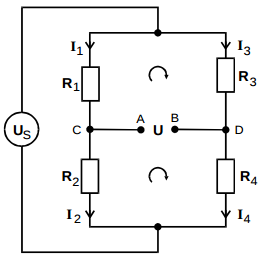
\includegraphics[width=0.5\textwidth]{V3021.png}
  \caption{Schaltplan der allgemeinen Brückenschaltung}
  \label{fig:V3021}
\end{figure}
In Abbildung \ref{fig:V3021} ist der Aufbau der allgemeinen
Brückenschaltung zu sehen. An den Punkten A und B wird die Brückenspannung abgegriffen.
Sie wird durch das Verhältnis der eingebrachten Widerstände $R_1$ und $R_4$
bestimmt.
Wenn die Abgleichbedingung
\begin{equation}
    R_1 R_4 = R_2 R_3
    \label{eq:abgleich}
\end{equation}
gegeben ist, ist eine Nullspannung erreicht. Für komplexe Widerstände folgt:
\begin{equation}
    Z = X + \mathup{i}Y.
\end{equation}
mit dem Wirkwiderstand X und dem Blindwiderstand Y. Die komplexen
Wechselstromwiderstände von einer idealen Kapazität $C$ und einer idealen
Induktivität $L$ sind, in Abhängigkeit von der Frequenz $\omega$, folgendermaßen
definiert:
\begin{equation}
    Z_C = -\frac{\mathup{i}}{\omega C} \quad \mathup{und} \quad Z_L = \mathup{i} \omega L.
    \label{eq:impedanzen}
\end{equation}
Zwei komplexe Zahlen sind nur dann gleich, wenn die Real- und die Imaginärteile
dieser gleich sind. Für komplexe Widerstände ergibt sich aus Gleichung
\ref{eq:abgleich} die Abgleichbedingung
\begin{equation}
    \label{eq:abgleich_komplex}
    Z_1 Z_4 = Z_2 Z_3.
\end{equation}
Damit folgt
\begin{align}
    \label{eq:abgleich_komplex_1}
    X_1 X_4 - Y_1 Y_4 &= X_2 X_3 - Y_2 Y_3 \\
    \shortintertext{und}
    \label{eq:abgleich_komplex_2}
    X_1 Y_4 + X_4 Y_1 &= X_2 Y_3 + X_3 Y_2.
\end{align}
\newpage
\subsection{Die Wheatstonesche Brücke}
\begin{figure}[htb]
  \centering
  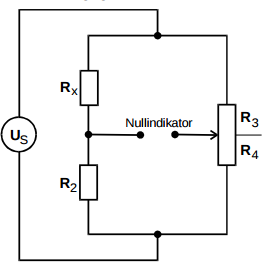
\includegraphics[width=0.5\textwidth]{V3022.png}
  \caption{Schaltplan der Wheatstoneschen Brücke}
  \label{fig:V3022}
\end{figure}
In Abbildung \ref{fig:V3022} zu sehen ist die Wheatstonesche Brückenschaltung.
Sie wird genutzt, um einen unbekannten ohmschen Widerstand $R_x$ zu bestimmen.
Bei einer Wheatstoneschen Brückenschaltung kann mit Gleich- und
Wechselstrom gearbeitet werden. Durch die Abgleichbeziehung ergibt sich,
dass durch die Änderung des Verhältnisses von $R_3$ und $R_4$ die
Brückenspannung auf 0 gebracht werden kann. Damit folgt
\begin{equation}
    \label{eq:wheatstone}
    R_{\mathup{x}} = R_2 \frac{R_3}{R_4}
\end{equation}
\newpage
\subsection{Die Kapazitätsmessbrücke}
\begin{figure}[htb]
  \centering
  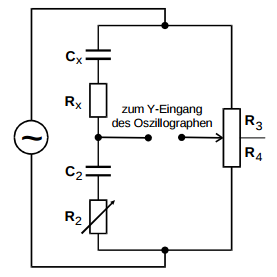
\includegraphics[width=0.5\textwidth]{V3023.png}
  \caption{Schaltplan der Kapazitätsmessbrücke}
  \label{fig:V3023}
\end{figure}
In Abbildung \ref{fig:V3023} zu sehen ist die Brückenschaltung für die
Kapazitätsmessbrücke. Nun wird der unbekannte Widerstand $R_x$ durch einen
Kondensator $C_x$ ersetzt. Da der Kondensator allerdings auch verlustbehaftet
ist, ist im Schaltbild \ref{fig:V3023} ein fiktiver Widerstand $R_x$
berücksichtigt. Aus den beiden vorherigen Ausgleichsbedingungen folgt für
die Kapazitätsmessbrücke der Zusammenhang
\begin{align}
    \label{eq:kapazitätsmessbrücke_R}
    R_{\mathup{x}} &= R_2 \frac{R_3}{R_4} \\
    \shortintertext{und}
    \label{eq:kapazitätsmessbrücke_C}
    C_{\mathup{x}} &= C_2 \frac{R_4}{R_3}.
\end{align}

\newpage
\subsection{Die Induktivitätsmessbrücke}
\begin{figure}[htb]
  \centering
  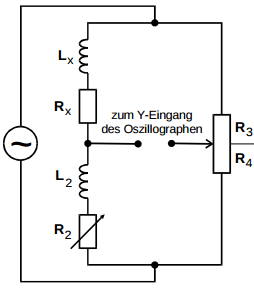
\includegraphics[width=0.5\textwidth]{V3024.png}
  \caption{Schaltplan der Induktivitätsmessbrücke}
  \label{fig:V3024}
\end{figure}
In Abbildung \ref{fig:V3024} zu sehen ist die Brückenschaltung für die
Induktivitätsmessbrücke. Induktivitäten werden dabei analog wie bei der
Kapazitätsmessbrücke bestimmt, mit dem Unterschied, dass die Kapazitäten
durch Induktivitäten ersetzt werden. Dabei folgen aus den Abgleichbedingungen
folgende Zusammenhänge:
\begin{align}
    \label{eq:induktivitätsmessbrücke_R}
    R_{\mathup{x}} &= R_2 \frac{R_3}{R_4} \\
    \label{eq:induktivitätsmessbrücke_L}
    L_{\mathup{x}} &= L_2 \frac{R_3}{R_4}.
\end{align}
\newpage
\subsection{Die Maxwell-Brücke}
\begin{figure}[htb]
  \centering
  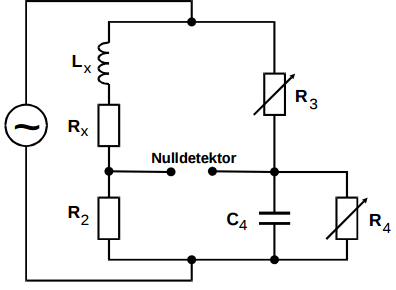
\includegraphics[width=0.5\textwidth]{V3025.png}
  \caption{Schaltplan der Maxwell-Brücke}
  \label{fig:V3025}
\end{figure}
In Abbildung \ref{fig:V3025} zu sehen ist die Brückenschaltung für die
Maxwell-Brücke. Hier wird auf die Induktivität $L_2$, welche bei der
Induktivitätsmessbrücke noch verwendet wurde, verzichtet. Stattdessen wird mit
einem Kondensator $C_4$ gearbeitet. Aus den Abgleichbedingungen folgen dann die
Beziehungen
\begin{align}
    \label{eq:maxwell_R}
    R_{\mathup{x}} &= \frac{R_2 R_3}{R_4} \\
    \shortintertext{und}
    \label{eq:maxwell_L}
    L_{\mathup{x}} &= R_2 R_3 C_4.
\end{align}

\newpage
\subsection{Die Wien-Robinson-Brücke}
\begin{figure}[htb]
  \centering
  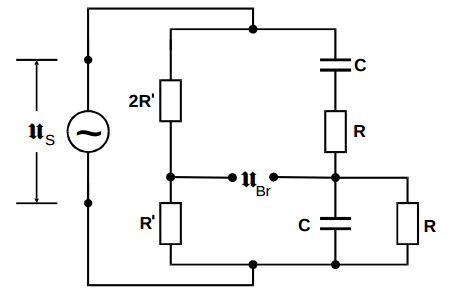
\includegraphics[width=0.5\textwidth]{V3026.png}
  \caption{Schaltplan der Wien-Robinson-Brücke}
  \label{fig:V3026}
\end{figure}
In Abbildung \ref{fig:V3026} zu sehen ist die Brückenschaltung für die
Wien-Robinson-Brücke. Nun werden keine unbekannten Induktivitäten, Widerstände
oder Kapazitäten mehr genutzt, sondern es wird die Frequenzabhängigkeit
untersucht. Die Wien-Robinson-Brücke fungiert als Sperrfilter. Ein Sperrfilter
foltert eine bestimmte Frequenz einer Spannungsquelle vollständig aus dem
Spektrum heraus. Das Verhältnis zwischen Brückenspannung $U$ und Quellspannung
$U_Q$ kann man mit Hilfe der Kirchhoffschen Regeln \ref{Knotenregel} als
\begin{equation}
    \label{eq:wien_robinson_1}
    \left|\frac{U}{U_{\mathup{S}}}\right|^2 = \frac{\left(\omega^2 R^2 C^2 - 1\right)^2}{9\left(\left(1 - \omega^2 R^2 C^2\right)^2 + 9 \omega^2 R^2 C^2\right)}.
\end{equation}

ausdrücken.
\newpage
\section{Durchführung}
\label{sec:durchführung}
\subsection{Widerstandsmessung}
Als erstes wird in dem Versuch mit einer Wheatstoneschen Brücke, wie in
Abbildung \ref{fig:V3022} dargestellt, gearbeitet. Sie ist an einer
Wechselstromspannungsquelle angeschlossen. Zu bestimmen ist der Widerstand $R_x$.
Dieser ist unbekannt. Um $R_x$ zu bestimmen, wird das am Potentiometer
regelbare Verhältnis der beiden Widerstände $R_3$ und $R_4$ so eingestellt, dass
der Oszillograph eine Nullspaannung anzeigt. Diese Messung wird an zwei
verschiedenen unbekannten Widerständen $R_x$ durchgeführt, mit drei verschiedenen
$R_2$-Widerständen, um die Messgenauigkeit zu verbessern.
\subsection{Kapazitätsmessung}
Als nächstes wird eine Kapazitätsmessung durchgeführt. Dafür verändert man die
Schaltung, wie in \ref{fig:V3023} dargestellt. Wie auch schon bei der
Widerstandsmessung wird erneut die Nullspannung gesucht. Diese Messung wird
für einen weiteren idealen Kondensator wiederholt. Bei der nächsten Messung wird ein Kondensator
verwendet, der einen Wirkanteil in seinem Widerstand hat. Auch hier
wird eine Nullspannung gesucht. Dabei wird so abwechselnd variiert, bis ein
absolutes Minimum nahe Null gefunden wird. Dabei werden beide eingestellten
Widerstände notiert. Außerdem wird jede Messung mit drei verschiedenen
Kapazitäten $C_2$ durchgeführt.
\newpage
\subsection{Induktivitätsmessung}
Als nächstes wird eine Induktivitätsmessung durchgeführt. Dafür wird ein Aufbau.
wie in Abbildung \ref{fig:V3024} zu sehen, genutzt. Diese Messung
ist, vom Ablauf her, analog zu der Kapazitätsmessung. Um hier eine bessere
Messgenauigkeit zu gewährleisten wird die Messung mit drei verschiedenen
$L_2$-Induktivitäten durchgeführt.
Daraufhin wird mit einer Maxwell-Brücke, wie in Abbildung \ref{fig:V3025} zu
sehen, dieselbe Induktivität, wie bei der ersten Induktivitätsmessung,
bestimmt. Die Werte werden für $R_3$ und $R_4$ bestimmt und die Messung wird
für zwei weitere $R_2$-Widerstände wiederholt.

\subsection{Untersuchung der Frequenzanhängigkeit einer Wien-Robinson-Brücke}
Als letztes wird die Frequenzabhängigkeit einer Brückenschaltung untersucht.
Dafür nutzt man eine Wien-Robinson-Brücke, wie in Abbildung \ref{fig:V3026}
zu sehen. Der in der Schaltung enthaltene Wechselstromgenerator liefert eine
Quellspannung $U_Q$. Diese Spannung hat eine variable bzw.
einstellbare Frequenz. Zur Messung wird dann die Brückenspannung $U$ gegen die
Frequenz $f$ zwischen \SI{20}{\hertz} und \SI{20}{\kilo\hertz} aufgenommen. Es
werden 37 Werte aufgenommen für die Frequenz, $U_Q$ und $U$. Dabei wird auf das
Spannungsminimum von $U$ besonders Wert gelegt, indem man vorallem Frequenzen
bestimmt, die nahe an dem Spannungsminimum von \SI{0.0152}{\volt} bei einer
Frequenz von \SI{378}{\hertz} liegen.
\newpage
\end{document}
